% Options for packages loaded elsewhere
\PassOptionsToPackage{unicode}{hyperref}
\PassOptionsToPackage{hyphens}{url}
%
\documentclass[
]{article}
\usepackage{lmodern}
\usepackage{amssymb,amsmath}
\usepackage{ifxetex,ifluatex}
\ifnum 0\ifxetex 1\fi\ifluatex 1\fi=0 % if pdftex
  \usepackage[T1]{fontenc}
  \usepackage[utf8]{inputenc}
  \usepackage{textcomp} % provide euro and other symbols
\else % if luatex or xetex
  \usepackage{unicode-math}
  \defaultfontfeatures{Scale=MatchLowercase}
  \defaultfontfeatures[\rmfamily]{Ligatures=TeX,Scale=1}
\fi
% Use upquote if available, for straight quotes in verbatim environments
\IfFileExists{upquote.sty}{\usepackage{upquote}}{}
\IfFileExists{microtype.sty}{% use microtype if available
  \usepackage[]{microtype}
  \UseMicrotypeSet[protrusion]{basicmath} % disable protrusion for tt fonts
}{}
\makeatletter
\@ifundefined{KOMAClassName}{% if non-KOMA class
  \IfFileExists{parskip.sty}{%
    \usepackage{parskip}
  }{% else
    \setlength{\parindent}{0pt}
    \setlength{\parskip}{6pt plus 2pt minus 1pt}}
}{% if KOMA class
  \KOMAoptions{parskip=half}}
\makeatother
\usepackage{xcolor}
\IfFileExists{xurl.sty}{\usepackage{xurl}}{} % add URL line breaks if available
\IfFileExists{bookmark.sty}{\usepackage{bookmark}}{\usepackage{hyperref}}
\hypersetup{
  pdftitle={Lab 6},
  pdfauthor={Yunting Chiu},
  hidelinks,
  pdfcreator={LaTeX via pandoc}}
\urlstyle{same} % disable monospaced font for URLs
\usepackage[margin=1in]{geometry}
\usepackage{color}
\usepackage{fancyvrb}
\newcommand{\VerbBar}{|}
\newcommand{\VERB}{\Verb[commandchars=\\\{\}]}
\DefineVerbatimEnvironment{Highlighting}{Verbatim}{commandchars=\\\{\}}
% Add ',fontsize=\small' for more characters per line
\usepackage{framed}
\definecolor{shadecolor}{RGB}{248,248,248}
\newenvironment{Shaded}{\begin{snugshade}}{\end{snugshade}}
\newcommand{\AlertTok}[1]{\textcolor[rgb]{0.94,0.16,0.16}{#1}}
\newcommand{\AnnotationTok}[1]{\textcolor[rgb]{0.56,0.35,0.01}{\textbf{\textit{#1}}}}
\newcommand{\AttributeTok}[1]{\textcolor[rgb]{0.77,0.63,0.00}{#1}}
\newcommand{\BaseNTok}[1]{\textcolor[rgb]{0.00,0.00,0.81}{#1}}
\newcommand{\BuiltInTok}[1]{#1}
\newcommand{\CharTok}[1]{\textcolor[rgb]{0.31,0.60,0.02}{#1}}
\newcommand{\CommentTok}[1]{\textcolor[rgb]{0.56,0.35,0.01}{\textit{#1}}}
\newcommand{\CommentVarTok}[1]{\textcolor[rgb]{0.56,0.35,0.01}{\textbf{\textit{#1}}}}
\newcommand{\ConstantTok}[1]{\textcolor[rgb]{0.00,0.00,0.00}{#1}}
\newcommand{\ControlFlowTok}[1]{\textcolor[rgb]{0.13,0.29,0.53}{\textbf{#1}}}
\newcommand{\DataTypeTok}[1]{\textcolor[rgb]{0.13,0.29,0.53}{#1}}
\newcommand{\DecValTok}[1]{\textcolor[rgb]{0.00,0.00,0.81}{#1}}
\newcommand{\DocumentationTok}[1]{\textcolor[rgb]{0.56,0.35,0.01}{\textbf{\textit{#1}}}}
\newcommand{\ErrorTok}[1]{\textcolor[rgb]{0.64,0.00,0.00}{\textbf{#1}}}
\newcommand{\ExtensionTok}[1]{#1}
\newcommand{\FloatTok}[1]{\textcolor[rgb]{0.00,0.00,0.81}{#1}}
\newcommand{\FunctionTok}[1]{\textcolor[rgb]{0.00,0.00,0.00}{#1}}
\newcommand{\ImportTok}[1]{#1}
\newcommand{\InformationTok}[1]{\textcolor[rgb]{0.56,0.35,0.01}{\textbf{\textit{#1}}}}
\newcommand{\KeywordTok}[1]{\textcolor[rgb]{0.13,0.29,0.53}{\textbf{#1}}}
\newcommand{\NormalTok}[1]{#1}
\newcommand{\OperatorTok}[1]{\textcolor[rgb]{0.81,0.36,0.00}{\textbf{#1}}}
\newcommand{\OtherTok}[1]{\textcolor[rgb]{0.56,0.35,0.01}{#1}}
\newcommand{\PreprocessorTok}[1]{\textcolor[rgb]{0.56,0.35,0.01}{\textit{#1}}}
\newcommand{\RegionMarkerTok}[1]{#1}
\newcommand{\SpecialCharTok}[1]{\textcolor[rgb]{0.00,0.00,0.00}{#1}}
\newcommand{\SpecialStringTok}[1]{\textcolor[rgb]{0.31,0.60,0.02}{#1}}
\newcommand{\StringTok}[1]{\textcolor[rgb]{0.31,0.60,0.02}{#1}}
\newcommand{\VariableTok}[1]{\textcolor[rgb]{0.00,0.00,0.00}{#1}}
\newcommand{\VerbatimStringTok}[1]{\textcolor[rgb]{0.31,0.60,0.02}{#1}}
\newcommand{\WarningTok}[1]{\textcolor[rgb]{0.56,0.35,0.01}{\textbf{\textit{#1}}}}
\usepackage{graphicx,grffile}
\makeatletter
\def\maxwidth{\ifdim\Gin@nat@width>\linewidth\linewidth\else\Gin@nat@width\fi}
\def\maxheight{\ifdim\Gin@nat@height>\textheight\textheight\else\Gin@nat@height\fi}
\makeatother
% Scale images if necessary, so that they will not overflow the page
% margins by default, and it is still possible to overwrite the defaults
% using explicit options in \includegraphics[width, height, ...]{}
\setkeys{Gin}{width=\maxwidth,height=\maxheight,keepaspectratio}
% Set default figure placement to htbp
\makeatletter
\def\fps@figure{htbp}
\makeatother
\setlength{\emergencystretch}{3em} % prevent overfull lines
\providecommand{\tightlist}{%
  \setlength{\itemsep}{0pt}\setlength{\parskip}{0pt}}
\setcounter{secnumdepth}{-\maxdimen} % remove section numbering

\title{Lab 6}
\author{Yunting Chiu}
\date{2021-02-12}

\begin{document}
\maketitle

\hypertarget{r-lab-6}{%
\section{R Lab 6}\label{r-lab-6}}

\hypertarget{exercise-1}{%
\section{Exercise 1}\label{exercise-1}}

\hypertarget{section}{%
\subsection{1.1}\label{section}}

\begin{itemize}
\tightlist
\item
  X is V2, which means the ACT test score.
\item
  Y is V1, which means the GPA at the end of the freshman year.
\end{itemize}

\begin{Shaded}
\begin{Highlighting}[]
\NormalTok{GPA =}\StringTok{ }\KeywordTok{read.table}\NormalTok{(}\StringTok{"./data/CH01PR19.txt"}\NormalTok{)}
\KeywordTok{attach}\NormalTok{(GPA)}
\NormalTok{X <-}\StringTok{ }\NormalTok{V2}
\NormalTok{Y <-}\StringTok{ }\NormalTok{V1}
\CommentTok{# X = ACT, Y = GPA}
\end{Highlighting}
\end{Shaded}

\hypertarget{section-1}{%
\subsection{1.2}\label{section-1}}

According to the plot below, we can see that many data points do not fit
the linear regression line.

\begin{Shaded}
\begin{Highlighting}[]
\NormalTok{reg =}\StringTok{ }\KeywordTok{lm}\NormalTok{(Y }\OperatorTok{~}\StringTok{ }\NormalTok{X)}
\NormalTok{reg}
\end{Highlighting}
\end{Shaded}

\begin{verbatim}
## 
## Call:
## lm(formula = Y ~ X)
## 
## Coefficients:
## (Intercept)            X  
##     2.11405      0.03883
\end{verbatim}

\begin{Shaded}
\begin{Highlighting}[]
\KeywordTok{plot}\NormalTok{(X, Y, }\DataTypeTok{xlab =} \StringTok{"x = ACT"}\NormalTok{, }\DataTypeTok{ylab =} \StringTok{"y = GPA"}\NormalTok{)}
\KeywordTok{abline}\NormalTok{(reg, }\DataTypeTok{col =} \StringTok{"red"}\NormalTok{)}
\end{Highlighting}
\end{Shaded}

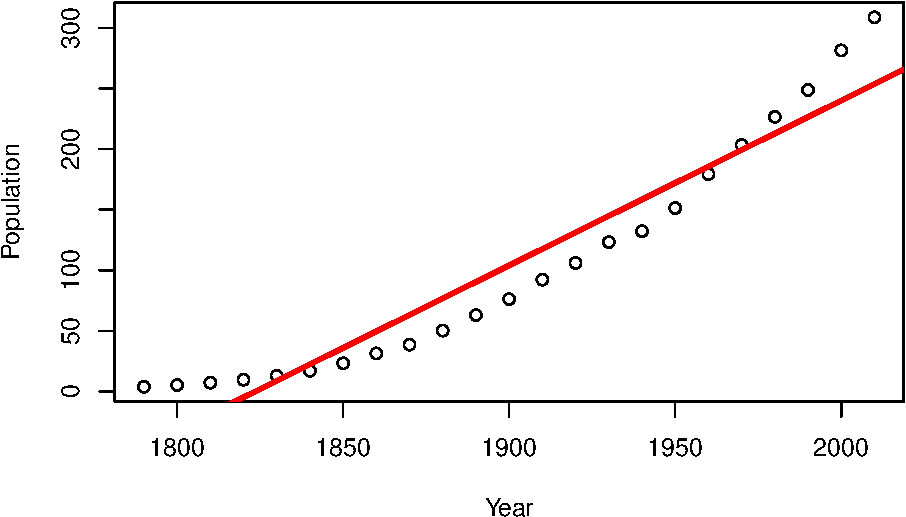
\includegraphics{lab6_files/figure-latex/unnamed-chunk-2-1.pdf}

\begin{Shaded}
\begin{Highlighting}[]
\CommentTok{# b0 =  2.11405   }
\CommentTok{# b1 = 0.03883  }
\end{Highlighting}
\end{Shaded}

\hypertarget{section-2}{%
\subsection{1.3}\label{section-2}}

We use \texttt{predict} function to estimate it. If ACT score is 30,
then the estimated mean of the freshman GPA would be 3.278863.

\begin{Shaded}
\begin{Highlighting}[]
\KeywordTok{predict}\NormalTok{(reg, }\KeywordTok{data.frame}\NormalTok{(}\DataTypeTok{X =} \DecValTok{30}\NormalTok{))}
\end{Highlighting}
\end{Shaded}

\begin{verbatim}
##        1 
## 3.278863
\end{verbatim}

\hypertarget{section-3}{%
\subsection{1.4}\label{section-3}}

The key is we should find b1. If the ACT score increases by one point,
we estimate GPA would be changed 0.03882713 units.

\begin{Shaded}
\begin{Highlighting}[]
\KeywordTok{summary}\NormalTok{(reg)}
\end{Highlighting}
\end{Shaded}

\begin{verbatim}
## 
## Call:
## lm(formula = Y ~ X)
## 
## Residuals:
##      Min       1Q   Median       3Q      Max 
## -2.74004 -0.33827  0.04062  0.44064  1.22737 
## 
## Coefficients:
##             Estimate Std. Error t value Pr(>|t|)    
## (Intercept)  2.11405    0.32089   6.588  1.3e-09 ***
## X            0.03883    0.01277   3.040  0.00292 ** 
## ---
## Signif. codes:  0 '***' 0.001 '**' 0.01 '*' 0.05 '.' 0.1 ' ' 1
## 
## Residual standard error: 0.6231 on 118 degrees of freedom
## Multiple R-squared:  0.07262,    Adjusted R-squared:  0.06476 
## F-statistic:  9.24 on 1 and 118 DF,  p-value: 0.002917
\end{verbatim}

\begin{Shaded}
\begin{Highlighting}[]
\NormalTok{reg}\OperatorTok{$}\NormalTok{coefficients[}\DecValTok{2}\NormalTok{]}
\end{Highlighting}
\end{Shaded}

\begin{verbatim}
##          X 
## 0.03882713
\end{verbatim}

\hypertarget{section-4}{%
\subsection{1.5}\label{section-4}}

\(e\) is the residuals. Another way is we can use \texttt{anova} table
to find out the residuals.

\begin{Shaded}
\begin{Highlighting}[]
\NormalTok{e =}\StringTok{ }\NormalTok{Y }\OperatorTok{-}\StringTok{ }\KeywordTok{fitted.values}\NormalTok{(reg)}
\NormalTok{e }\CommentTok{# ei each}
\end{Highlighting}
\end{Shaded}

\begin{verbatim}
##           1           2           3           4           5           6 
##  0.96758105  1.22737094  0.57679116 -0.42824608  0.09858105  0.54730978 
##           7           8           9          10          11          12 
## -0.39451735  0.79861829 -2.74003597  0.05444541  0.26409967  0.25913691 
##          13          14          15          16          17          18 
##  0.03709967 -0.03290033 -0.15034448 -0.19938171  0.43727254 -0.30469022 
##          19          20          21          22          23          24 
## -0.13772746 -0.77259183 -0.48290033  0.42758105  0.52979116  0.76261829 
##          25          26          27          28          29          30 
##  0.35479116 -0.02255459 -0.78120884 -0.38924608  0.74744541  0.13058105 
##          31          32          33          34          35          36 
##  0.84227254 -0.36028332 -0.27220884  0.25144541 -0.11124608  0.02609967 
##          37          38          39          40          41          42 
##  0.45158105  0.01113691  0.38661829  0.52244541 -0.14555459 -0.62486309 
##          43          44          45          46          47          48 
## -0.50590033 -0.87355459 -1.17103597 -0.42890033 -1.13469022 -0.69645619 
##          49          50          51          52          53          54 
##  0.10023530  0.99306243 -0.29138171  0.61671668  0.14261829 -0.17155459 
##          55          56          57          58          59          60 
##  0.50109967  0.41213691  0.23058105 -0.69659183  0.04413691  0.69596403 
##          61          62          63          64          65          66 
## -0.16272746 -0.29107321  0.28527254  0.59892679 -0.63686309 -0.47741895 
##          67          68          69          70          71          72 
## -0.39090033  0.35748265 -1.00693757  0.50892679  0.14840817 -0.04107321 
##          73          74          75          76          77          78 
## -0.33093757 -0.11293757  0.67996403 -0.05659183  0.21492679 -0.03955459 
##          79          80          81          82          83          84 
##  0.79879116  0.07682840  0.43240817  0.18140817 -1.04455459  0.51848265 
##          85          86          87          88          89          90 
##  0.12327254 -0.24238171  0.18261829  0.71596403  0.95623530 -0.42341895 
##          91          92          93          94          95          96 
##  0.84009967 -0.97938171  0.34427254  0.21106243  0.50996403  0.78709967 
##          97          98          99         100         101         102 
## -0.04938171 -0.05441895 -0.10476470 -0.50193757 -1.24372746 -1.22993757 
##         103         104         105         106         107         108 
## -0.01159183  0.23448265 -0.13190033  0.24300127 -0.28472746  0.41979116 
##         109         110         111         112         113         114 
##  0.59079116 -0.21772746  0.45075392  0.32113691 -0.49659183 -0.60459183 
##         115         116         117         118         119         120 
## -1.83169022  0.99440817  0.55996403  0.71279116 -0.87528332 -0.25320884
\end{verbatim}

\begin{Shaded}
\begin{Highlighting}[]
\KeywordTok{sum}\NormalTok{(e}\OperatorTok{^}\DecValTok{2}\NormalTok{) }\CommentTok{# sum of the squared residuals }
\end{Highlighting}
\end{Shaded}

\begin{verbatim}
## [1] 45.81761
\end{verbatim}

\begin{Shaded}
\begin{Highlighting}[]
\KeywordTok{anova}\NormalTok{(reg)}
\end{Highlighting}
\end{Shaded}

\begin{verbatim}
## Analysis of Variance Table
## 
## Response: Y
##            Df Sum Sq Mean Sq F value   Pr(>F)   
## X           1  3.588  3.5878  9.2402 0.002917 **
## Residuals 118 45.818  0.3883                    
## ---
## Signif. codes:  0 '***' 0.001 '**' 0.01 '*' 0.05 '.' 0.1 ' ' 1
\end{verbatim}

\hypertarget{section-5}{%
\subsection{1.6}\label{section-5}}

estimated variance is 0.3882848, and residual standard error: 0.6231 on
118 degrees of freedom

\begin{Shaded}
\begin{Highlighting}[]
\NormalTok{n <-}\StringTok{ }\KeywordTok{length}\NormalTok{(X)}
\NormalTok{var_est <-}\StringTok{ }\KeywordTok{sum}\NormalTok{(e}\OperatorTok{^}\DecValTok{2}\NormalTok{)}\OperatorTok{/}\NormalTok{(n}\DecValTok{-2}\NormalTok{) }\CommentTok{# sum of the squared residuals - degrees of freedom (n -2, b0 and b1 so minus 2)}
\NormalTok{var_est}
\end{Highlighting}
\end{Shaded}

\begin{verbatim}
## [1] 0.3882848
\end{verbatim}

\begin{Shaded}
\begin{Highlighting}[]
\KeywordTok{sqrt}\NormalTok{(var_est)}
\end{Highlighting}
\end{Shaded}

\begin{verbatim}
## [1] 0.623125
\end{verbatim}

\begin{Shaded}
\begin{Highlighting}[]
\KeywordTok{summary}\NormalTok{(reg)}
\end{Highlighting}
\end{Shaded}

\begin{verbatim}
## 
## Call:
## lm(formula = Y ~ X)
## 
## Residuals:
##      Min       1Q   Median       3Q      Max 
## -2.74004 -0.33827  0.04062  0.44064  1.22737 
## 
## Coefficients:
##             Estimate Std. Error t value Pr(>|t|)    
## (Intercept)  2.11405    0.32089   6.588  1.3e-09 ***
## X            0.03883    0.01277   3.040  0.00292 ** 
## ---
## Signif. codes:  0 '***' 0.001 '**' 0.01 '*' 0.05 '.' 0.1 ' ' 1
## 
## Residual standard error: 0.6231 on 118 degrees of freedom
## Multiple R-squared:  0.07262,    Adjusted R-squared:  0.06476 
## F-statistic:  9.24 on 1 and 118 DF,  p-value: 0.002917
\end{verbatim}

\hypertarget{exercise-2}{%
\section{Exercise 2}\label{exercise-2}}

\hypertarget{section-6}{%
\subsection{2.1}\label{section-6}}

Zero is not included, because the b1 is {[}0.005385614, 0.07226864{]}.

\begin{Shaded}
\begin{Highlighting}[]
\KeywordTok{confint}\NormalTok{(reg, }\DataTypeTok{level =} \FloatTok{0.99}\NormalTok{)}
\end{Highlighting}
\end{Shaded}

\begin{verbatim}
##                   0.5 %     99.5 %
## (Intercept) 1.273902675 2.95419590
## X           0.005385614 0.07226864
\end{verbatim}

\hypertarget{section-7}{%
\subsection{2.2}\label{section-7}}

\begin{itemize}
\tightlist
\item
  Ho: β1 = 0 (have NOT a linear association between ACT score (X) and
  GPA at the end of the freshman year (Y)).
\item
  Ha: β1 ≠ 0 (have a linear association between ACT score (X) and GPA at
  the end of the freshman year (Y)).
\end{itemize}

According to tables of a linear regression model above, we have evidence
to reject the null hypothesis in favor of the alternative hypothesis
with the 99 \% confidence interval. Thus, there is a linear association
between student's ACT score (X) and GPA at the end of the freshman year
(Y).

\hypertarget{section-8}{%
\subsection{2.3}\label{section-8}}

For the actual \textbf{population mean} response - confidence intervals

If ACT score is 28, wehave 95\% certain contains the population mean of
freshman GPA is 3.061384 to 3.341033.

\begin{Shaded}
\begin{Highlighting}[]
\KeywordTok{predict}\NormalTok{(reg, }\KeywordTok{data.frame}\NormalTok{(}\DataTypeTok{X =} \DecValTok{28}\NormalTok{), }\DataTypeTok{interval =} \StringTok{"confidence"}\NormalTok{, }\DataTypeTok{level =} \FloatTok{0.95}\NormalTok{)}
\end{Highlighting}
\end{Shaded}

\begin{verbatim}
##        fit      lwr      upr
## 1 3.201209 3.061384 3.341033
\end{verbatim}

\hypertarget{section-9}{%
\subsection{2.4}\label{section-9}}

For the individual response (actual response) \(Y\) - prediction
intervals

If student obtained a 28 on the ACT, the 95 \% prediction interval is
1.959355 to 4.443063 of his freshman GPA.

\begin{Shaded}
\begin{Highlighting}[]
\KeywordTok{predict}\NormalTok{(reg, }\KeywordTok{data.frame}\NormalTok{(}\DataTypeTok{X =} \DecValTok{28}\NormalTok{), }\DataTypeTok{interval =} \StringTok{"prediction"}\NormalTok{)}
\end{Highlighting}
\end{Shaded}

\begin{verbatim}
##        fit      lwr      upr
## 1 3.201209 1.959355 4.443063
\end{verbatim}

\hypertarget{section-10}{%
\subsection{2.5}\label{section-10}}

The majority of data points are in the range of upper band and lower
band. We can conclude that the true regression relation has been
precisely estimated.

\begin{Shaded}
\begin{Highlighting}[]
\NormalTok{n =}\StringTok{ }\KeywordTok{length}\NormalTok{(X) }\CommentTok{#sample sizes}
\NormalTok{e =}\StringTok{ }\NormalTok{reg}\OperatorTok{$}\NormalTok{residuals }\CommentTok{# residuals}
\NormalTok{s =}\StringTok{ }\KeywordTok{sqrt}\NormalTok{(}\KeywordTok{sum}\NormalTok{(e}\OperatorTok{^}\DecValTok{2}\NormalTok{)}\OperatorTok{/}\NormalTok{(n}\DecValTok{-2}\NormalTok{)) }\CommentTok{# estimated standard deviation = root MSE}
\NormalTok{s}
\end{Highlighting}
\end{Shaded}

\begin{verbatim}
## [1] 0.623125
\end{verbatim}

\begin{Shaded}
\begin{Highlighting}[]
\NormalTok{W =}\StringTok{ }\KeywordTok{sqrt}\NormalTok{(}\KeywordTok{qf}\NormalTok{(}\FloatTok{0.95}\NormalTok{,}\DecValTok{2}\NormalTok{,n}\DecValTok{-2}\NormalTok{))  }\CommentTok{# quantity of F-distribution}
\NormalTok{W}
\end{Highlighting}
\end{Shaded}

\begin{verbatim}
## [1] 1.753023
\end{verbatim}

\begin{Shaded}
\begin{Highlighting}[]
\NormalTok{Yhat =}\StringTok{ }\KeywordTok{fitted.values}\NormalTok{(reg) }\CommentTok{# Yhat = b0 + b1x = predict(reg)}
\NormalTok{Sxx =}\StringTok{ }\NormalTok{(n}\DecValTok{-1}\NormalTok{)}\OperatorTok{*}\KeywordTok{var}\NormalTok{(X) }

\NormalTok{margin =}\StringTok{ }\NormalTok{W}\OperatorTok{*}\NormalTok{s}\OperatorTok{*}\KeywordTok{sqrt}\NormalTok{(}\DecValTok{1}\OperatorTok{/}\NormalTok{n }\OperatorTok{+}\StringTok{ }\NormalTok{(X }\OperatorTok{-}\StringTok{ }\KeywordTok{mean}\NormalTok{(X))}\OperatorTok{^}\DecValTok{2}\OperatorTok{/}\NormalTok{Sxx) }
\NormalTok{upper.band =}\StringTok{ }\NormalTok{Yhat }\OperatorTok{+}\StringTok{ }\NormalTok{W}\OperatorTok{*}\NormalTok{s}\OperatorTok{*}\KeywordTok{sqrt}\NormalTok{(}\DecValTok{1} \OperatorTok{+}\StringTok{ }\DecValTok{1}\OperatorTok{/}\NormalTok{n }\OperatorTok{+}\StringTok{ }\NormalTok{(X }\OperatorTok{-}\StringTok{ }\KeywordTok{mean}\NormalTok{(X))}\OperatorTok{^}\DecValTok{2}\OperatorTok{/}\NormalTok{Sxx) }
\NormalTok{lower.band =}\StringTok{ }\NormalTok{Yhat }\OperatorTok{-}\StringTok{ }\NormalTok{W}\OperatorTok{*}\NormalTok{s}\OperatorTok{*}\KeywordTok{sqrt}\NormalTok{(}\DecValTok{1} \OperatorTok{+}\StringTok{ }\DecValTok{1}\OperatorTok{/}\NormalTok{n }\OperatorTok{+}\StringTok{ }\NormalTok{(X }\OperatorTok{-}\StringTok{ }\KeywordTok{mean}\NormalTok{(X))}\OperatorTok{^}\DecValTok{2}\OperatorTok{/}\NormalTok{Sxx) }

\KeywordTok{plot}\NormalTok{(X,Y,}\DataTypeTok{xlab=}\StringTok{"ACT"}\NormalTok{, }\DataTypeTok{ylab=}\StringTok{"Y = GPA"}\NormalTok{, }\DataTypeTok{xlim =} \KeywordTok{c}\NormalTok{(}\DecValTok{20}\NormalTok{,}\DecValTok{30}\NormalTok{))}
\KeywordTok{abline}\NormalTok{(reg,}\DataTypeTok{col=}\StringTok{"red"}\NormalTok{)}
\KeywordTok{lines}\NormalTok{(X,upper.band,}\DataTypeTok{col=}\StringTok{"blue"}\NormalTok{)}
\KeywordTok{lines}\NormalTok{(X,lower.band,}\DataTypeTok{col=}\StringTok{"blue"}\NormalTok{)}
\end{Highlighting}
\end{Shaded}

\includegraphics{lab6_files/figure-latex/unnamed-chunk-10-1.pdf}

\end{document}
